If the phase portrait changes its topological structure (loses topological equivalence\footnote{Intuitively, two phase portraits are \emph{topologically equivalent} if one is a distorted version of the other. Bending and warping are allowed, but not ripping, so closed orbits must remain closed, trajectories connecting saddle points must not be broken, etc.}) as a parameter is varied, we say that a bifurcation has occurred.
\subsection{Codimension of a Bifurcation}
The codimension of a bifurcation is the \emph{number of parameters} which must be varied for the bifurcation to occur.
This corresponds to the codimension of the parameter set for which the bifurcation occurs within the full space of parameters.
\subsection{Local Bifurcations}{\label{sec:lb}}
A \emph{local} bifurcation occurs when a parameter change causes the stability of an equilibrium (or fixed point) to change.
In continuous systems, this corresponds to the real part of an eigenvalue of an equilibrium passing through zero.
In discrete systems (those described by maps rather than ODEs) (See Section (\ref{sec:dds})), this corresponds to a fixed point having a \emph{Floquet multiplier} with modulus equal to one.
In both cases, the equilibrium is \emph{non-hyperbolic} at the bifurcation point.
The topological changes in the phase portrait of the system can be confined to arbitrarily small neighbourhoods of the bifurcating fixed points by moving the bifurcation parameter close to the bifurcation point (hence \emph{local}).\\\\
\textbullet\quad\textbf{Bifurcations at $\lambda_1=0$ or $\lambda_2=0$}
\subsubsection{Saddle-Node Bifurcation}{\label{sec:snbf2}}
The prototypical example in two dimensions is given by
\begin{equation}
	\begin{aligned}
		\dot{x}&=\mu-x^2\\
		\dot{y}&=-y
	\end{aligned}
\end{equation}
Consider the phase portrait as $\mu$ varies.
For $\mu=0$, Figure (\ref{fig:snbf2}) shows that there are two fixed points, a stable node at $(\tilde{x},\tilde{y})=(\sqrt{\mu},0)$ and a saddle at $(-\sqrt{\mu},0)$.
\begin{figure}[h!]
	\centering
	\begin{subfigure}{0.45\linewidth}
		\centering
		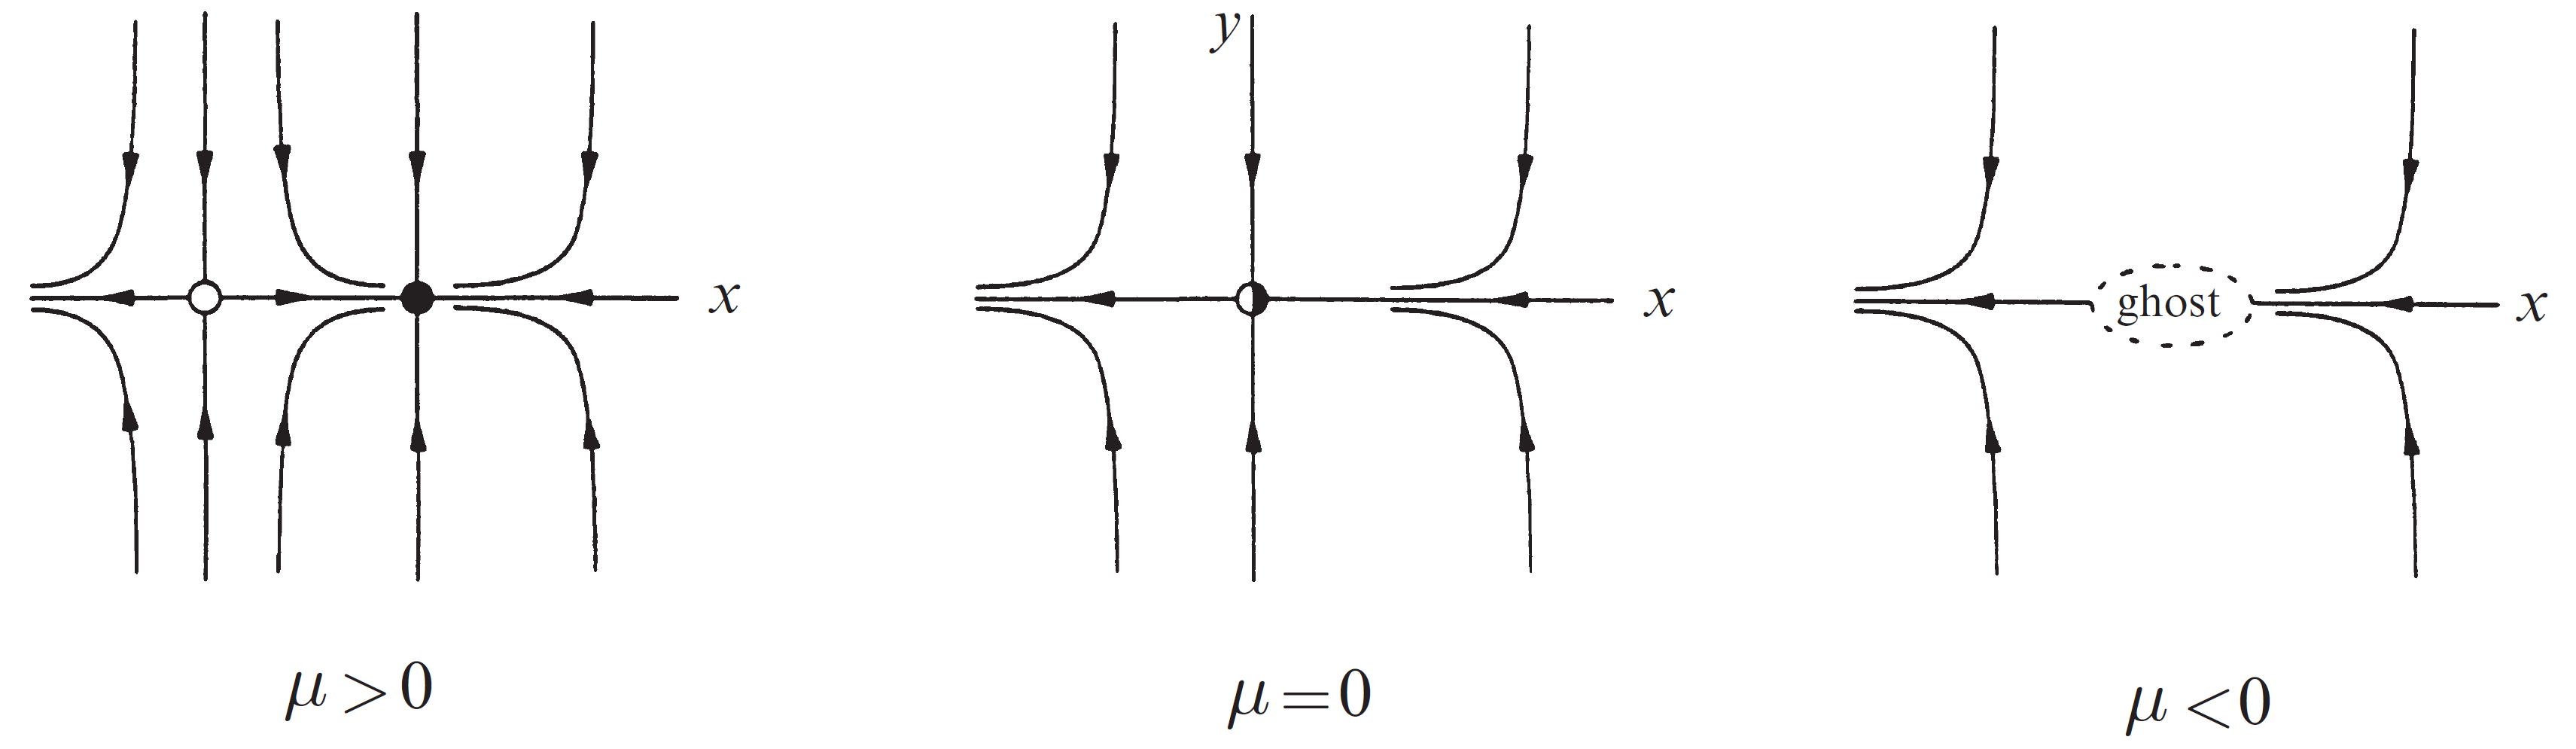
\includegraphics[width=\linewidth]{snbf2.png}
		\caption{Saddle-Node Bifurcation}
		\label{fig:snbf2}
	\end{subfigure}
	\vline
	\begin{subfigure}{0.42\linewidth}
		\centering
		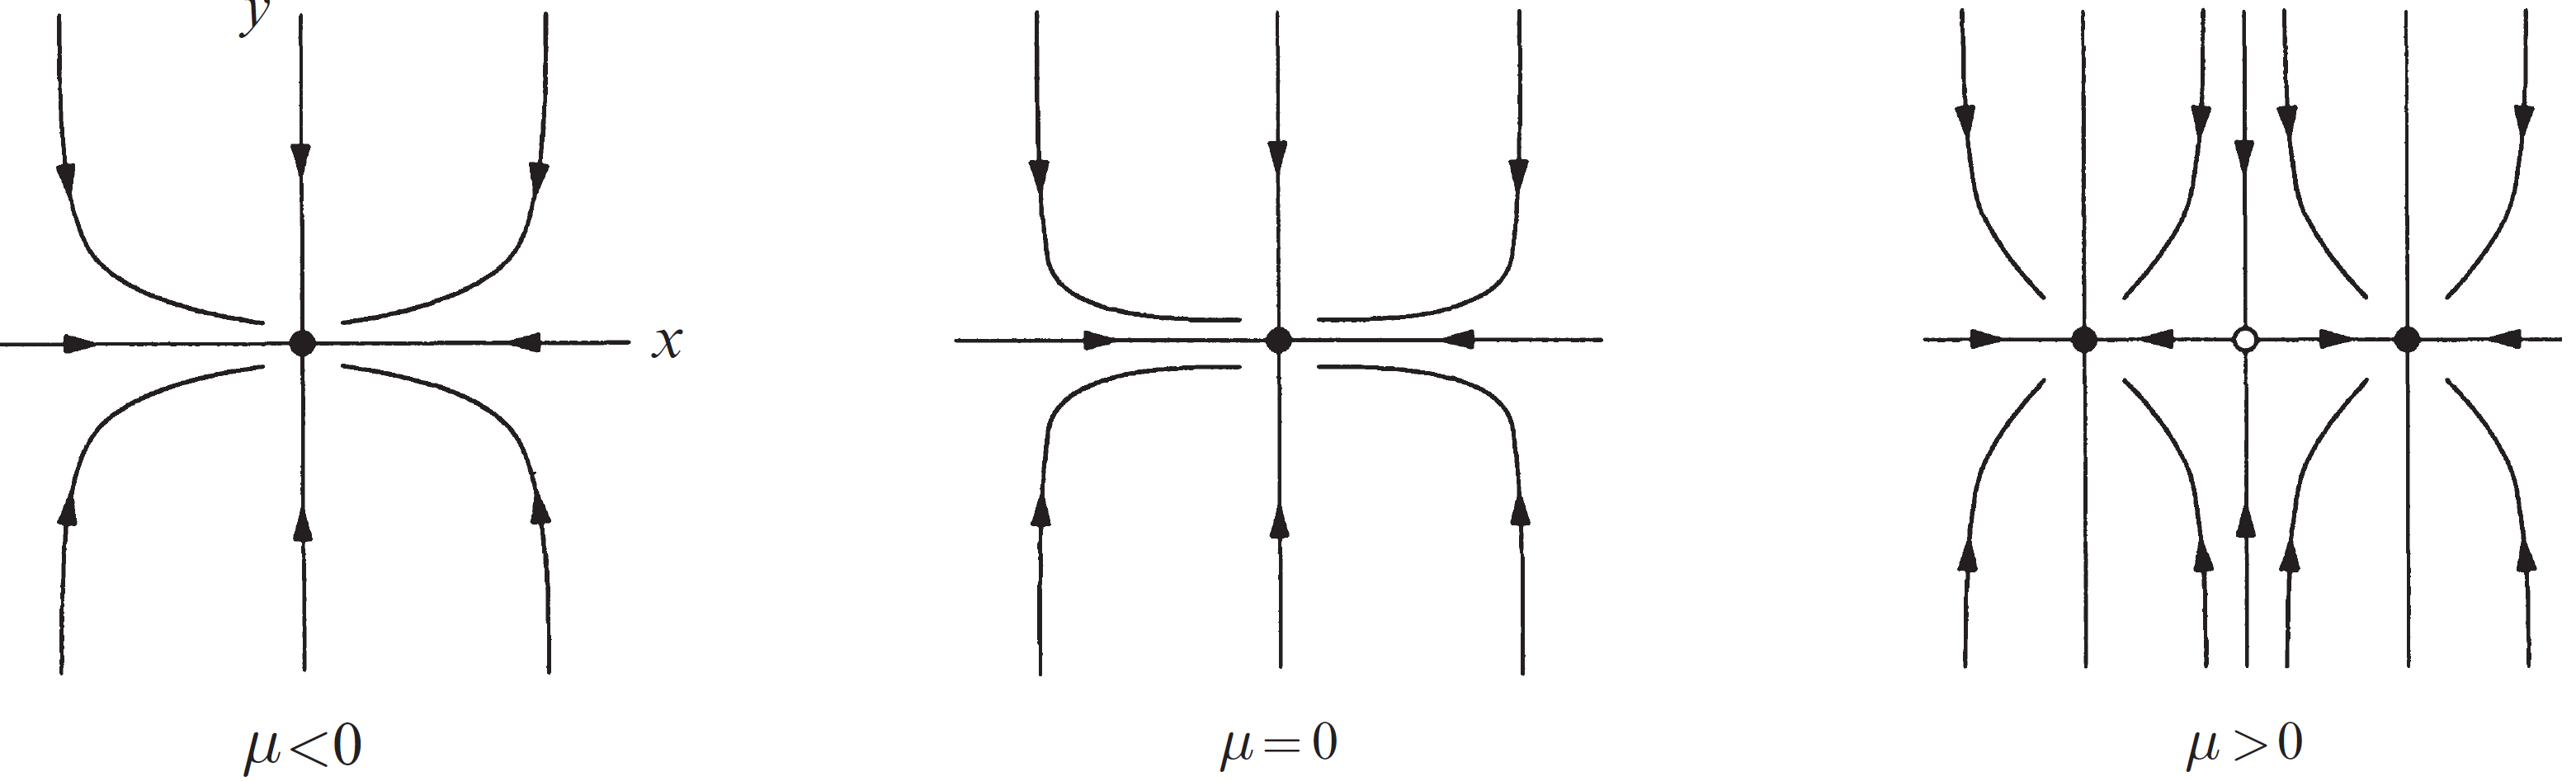
\includegraphics[width=\linewidth]{spbf2.png}
		\caption{Supercritical Pitchfork Bifurcation}
		\label{fig:spbf2}
	\end{subfigure}
	\caption{}
\end{figure}
As $\mu$ decreases, the saddle and node approach each other, then collide when $\mu=0$ and finally disappear when $\mu<0$.
Even after the fixed points have annihilated each other, they continue to influence the flow as in Section (\ref{sec:nuo}), they leave a \emph{ghost}, a bottleneck region that sucks trajectories in and delays them before allowing passage out the other side.
\subsubsection{Transcritical Bifurcation}
The prototypical example in two dimensions is given by
\begin{equation}
\begin{aligned}
\dot{x}&=\mu x-x^2\\
\dot{y}&=-y
\end{aligned}
\end{equation}
This system has always two distinct fixed points $(0,0)$ and $(\mu,0)$ for $\mu\neq0$. For $\mu=0$, these two fixed points merge at $(0, 0)$.
\begin{comment}
	\begin{figure}[h!]
	\centering
	\begin{subfigure}{0.45\linewidth}
	\centering
	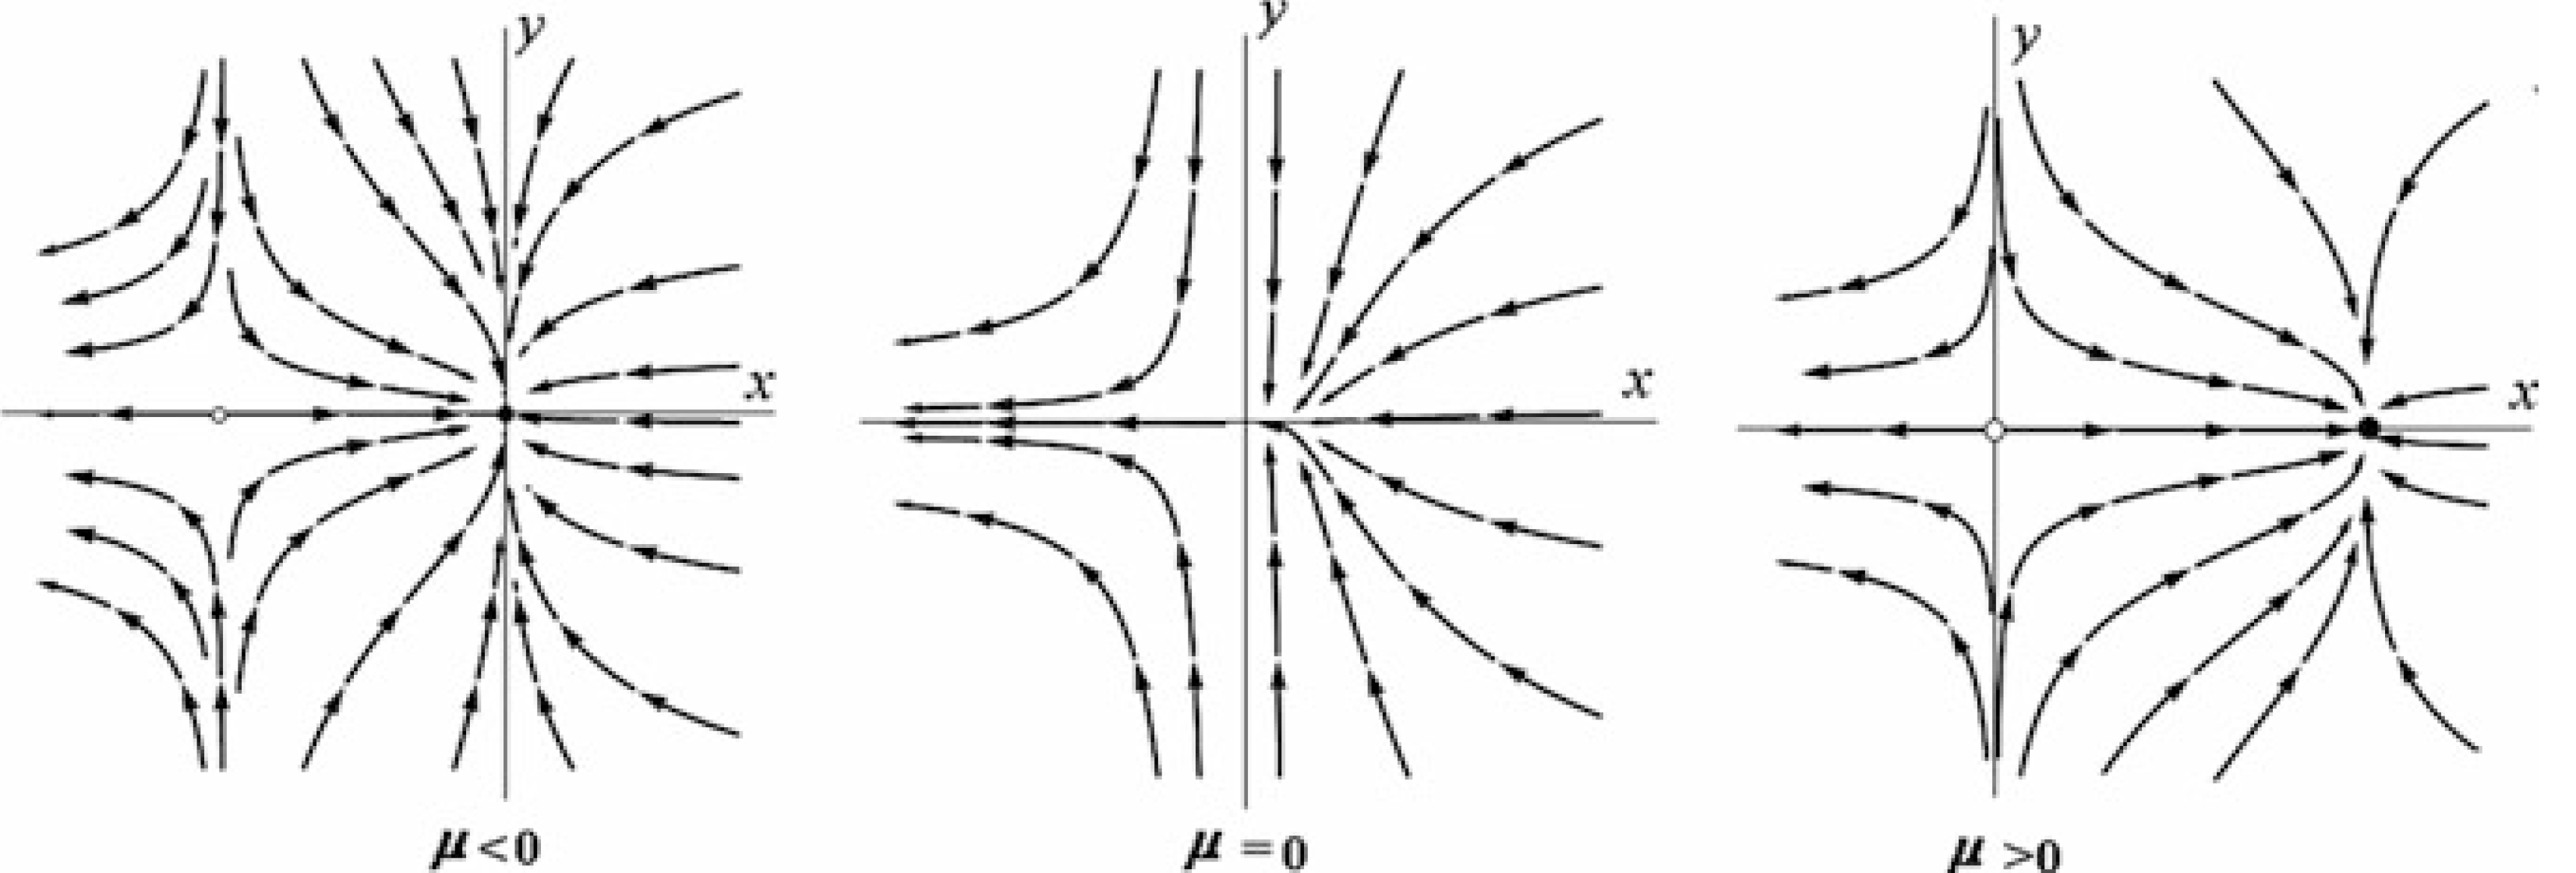
\includegraphics[width=\linewidth]{tbf2.png}
	\caption{Transcritical Bifurcation}
	\label{fig:tbf2}
	\end{subfigure}
	\vline
	\begin{subfigure}{0.45\linewidth}
	\centering
	\includegraphics[width=\linewidth]{sbbf2.png}
	\caption{Subcritical Pitchfork Bifurcation}
	\label{fig:sbbf2}
	\end{subfigure}
	\caption{}
	\end{figure}
\end{comment}
From the Phase portrait, we see that the behavior of the system changes when the parameter $\mu$ passes through the origin.
When $\mu$ passes through the origin from left, the fixed point origin changes to a saddle from a stable node and the fixed point $(\mu,0)$ changes from a saddle to a stable node.
\subsubsection{Supercritical Pitchfork Bifurcation}
The prototypical example in two dimensions is given by
\begin{equation}
	\begin{aligned}
		\dot{x}&=\mu x-x^3\\
		\dot{y}&=-y
	\end{aligned}
\end{equation}
For $\mu<0$, the only fixed point is a stable node at the origin. For $\mu=0$, the origin is still stable, but now we have very slow (algebraic) decay along the x-direction instead of exponential decay.
For $\mu>0$, the origin loses stability (becomes a saddle) and gives birth to two new stable fixed points symmetrically located at $(\pm\sqrt{\mu},0)$
\subsubsection{Subcritical Pitchfork Bifurcation}
The prototypical example in two dimensions is given by
\begin{equation}
	\begin{aligned}
		\dot{x}&=\mu x+x^3\\
		\dot{y}&=-y
	\end{aligned}
\end{equation}
\textbullet\quad\textbf{Hopf Bifurcations at $\lambda_{1,2}=\pm i\omega$}
\subsubsection{Supercritical Hopf bifurcation}
We consider the dynamical system
\begin{equation}{\label{eq:sphb}}
	\dot{\xi}=\mu\ \xi-\xi\ |\xi|^2\quad\text{with}\quad\mu,\xi\in\mathbb{C}\quad\text{Let}\quad
	\begin{cases}
		\mu=\epsilon+i\omega\\
		\xi=x+iy
	\end{cases}
\end{equation}
We see that (\ref{eq:sphb}) is indeed a two-dimensional dynamical system
\begin{equation}
	\begin{aligned}
		\dot{x}&=\epsilon x-\omega y-x(x^2+y^2)\\
		\dot{y}&=\omega x+\epsilon y-y(x^2+y^2)
	\end{aligned}\quad\rightarrow\quad
	\begin{aligned}
		\dot{r}&=\epsilon r-r^3\\
		\dot{\varphi}&=\omega
	\end{aligned}
\end{equation}
\begin{wrapfigure}{r}{0.4\linewidth}
	\centering
	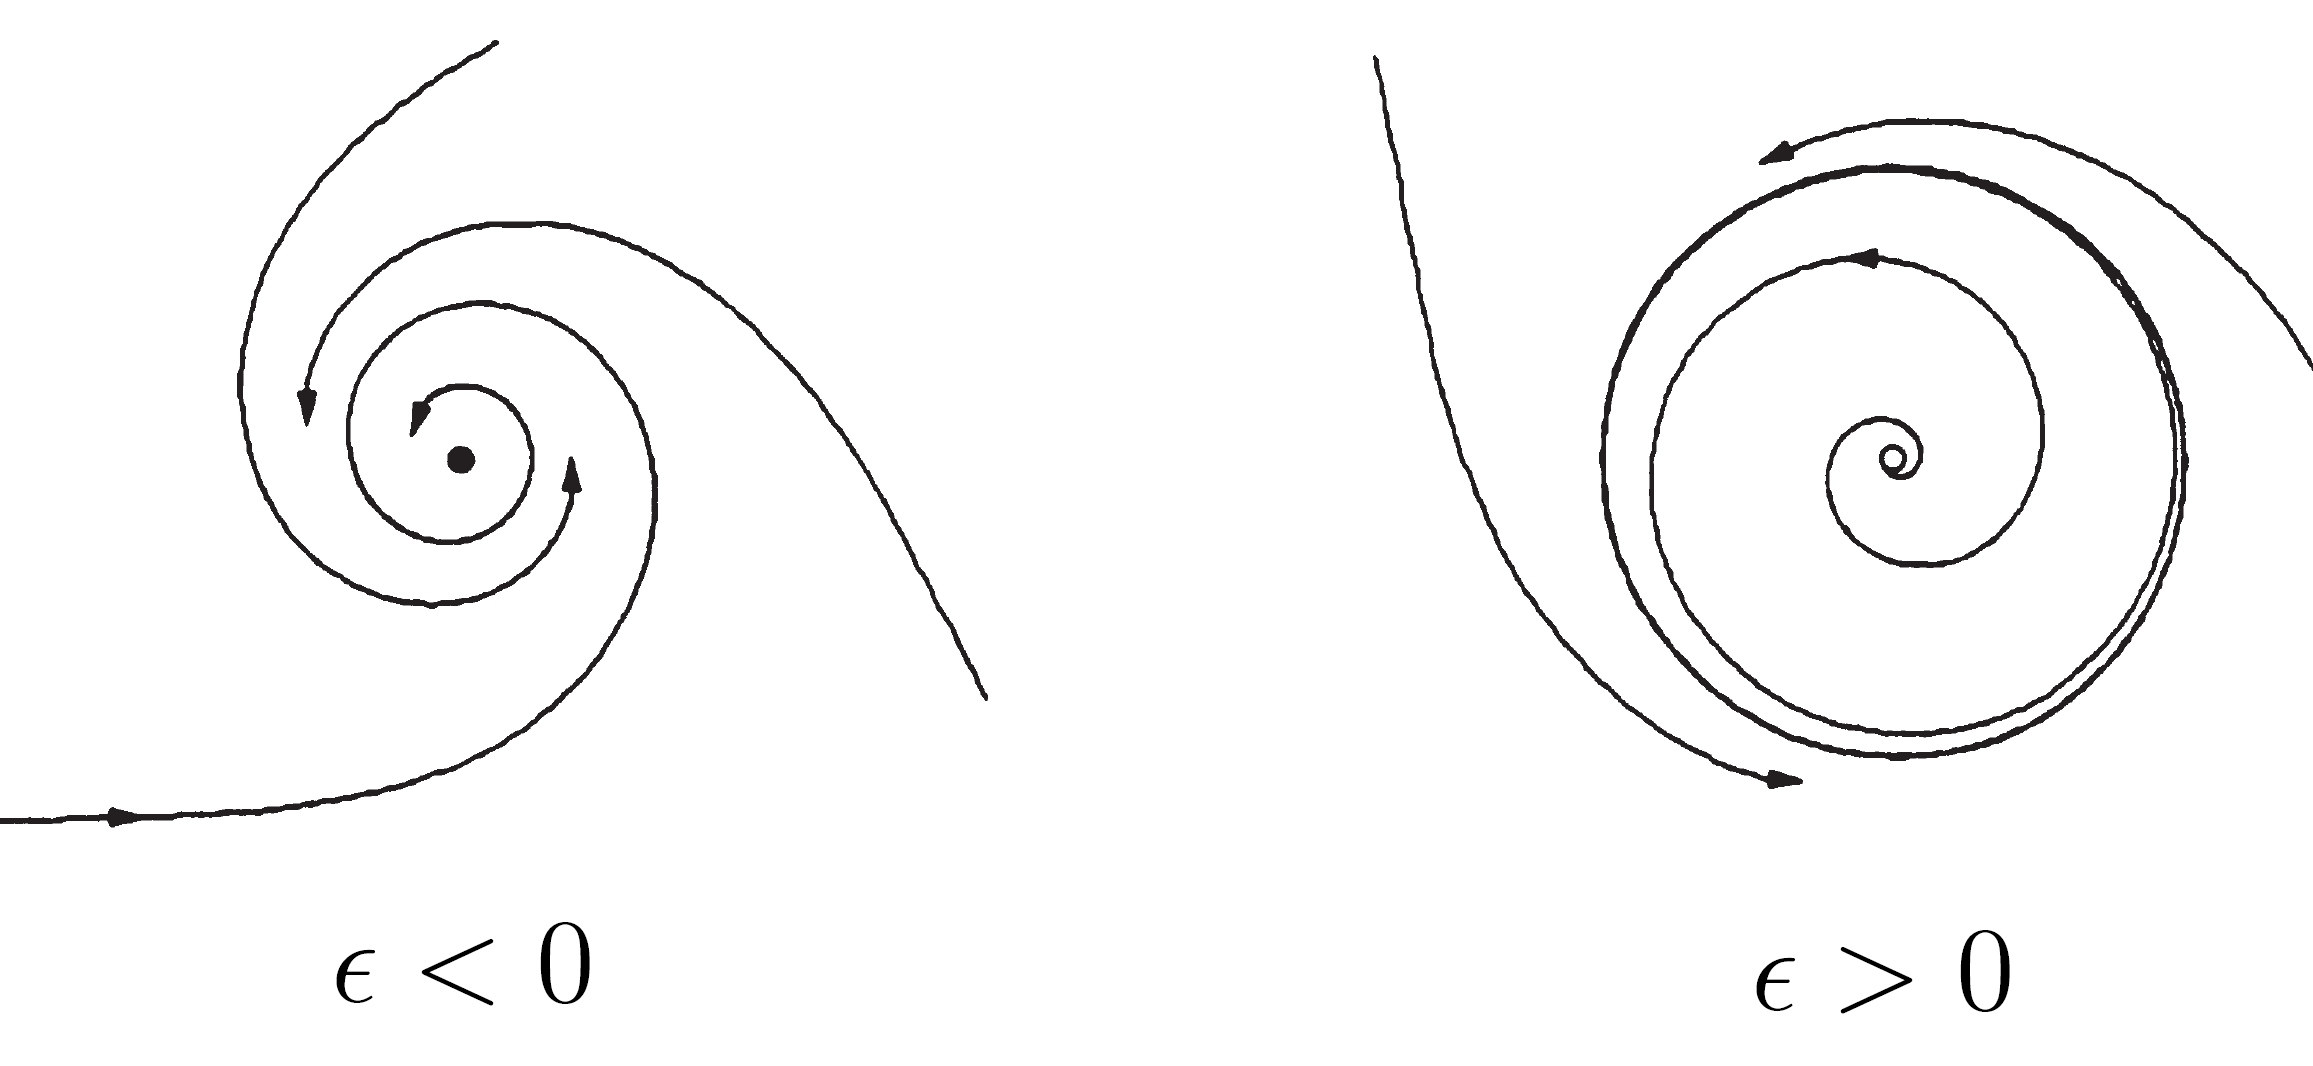
\includegraphics[width=\linewidth]{sphbf.png}
	\caption{Supercritical Hopf bifurcation}
	\label{fig:sphbf}
\end{wrapfigure}
As we have seen earlier (Equation (\ref{eq:spbf})), this equation has a single stable fixed point $r=0$ for $\epsilon<0$ and undergoes a supercritical pitchfork bifurcation at $\epsilon=0$, which turns this fixed point unstable and gives rise to two new stable fixed points at $r=\pm\sqrt{\epsilon}$.
Interpreting $r$ as the radius of a limit cycle, we find that a stable limit cycle with radius $\sqrt{\epsilon}$ arises from a fixed point when $\epsilon$ exceeds its critical value $\epsilon=0$.
\begin{equation}{\label{eq:sphbf}}
	\begin{pmatrix}
		\dot{x}\\\dot{y}
	\end{pmatrix}=
	\begin{pmatrix}
		\epsilon&-\omega\\
		\omega&\epsilon
	\end{pmatrix}=
	\begin{pmatrix}
		x\\y
	\end{pmatrix}
\end{equation}
The eigenvalues $\lambda$ for the matrix in (\ref{eq:sphbf}) are
\begin{equation}
	\lambda_{1,2}=\epsilon\pm i\omega
\end{equation}
\begin{comment}
	\begin{figure}[h!]
	\centering
	\begin{subfigure}{0.45\linewidth}
	\centering
	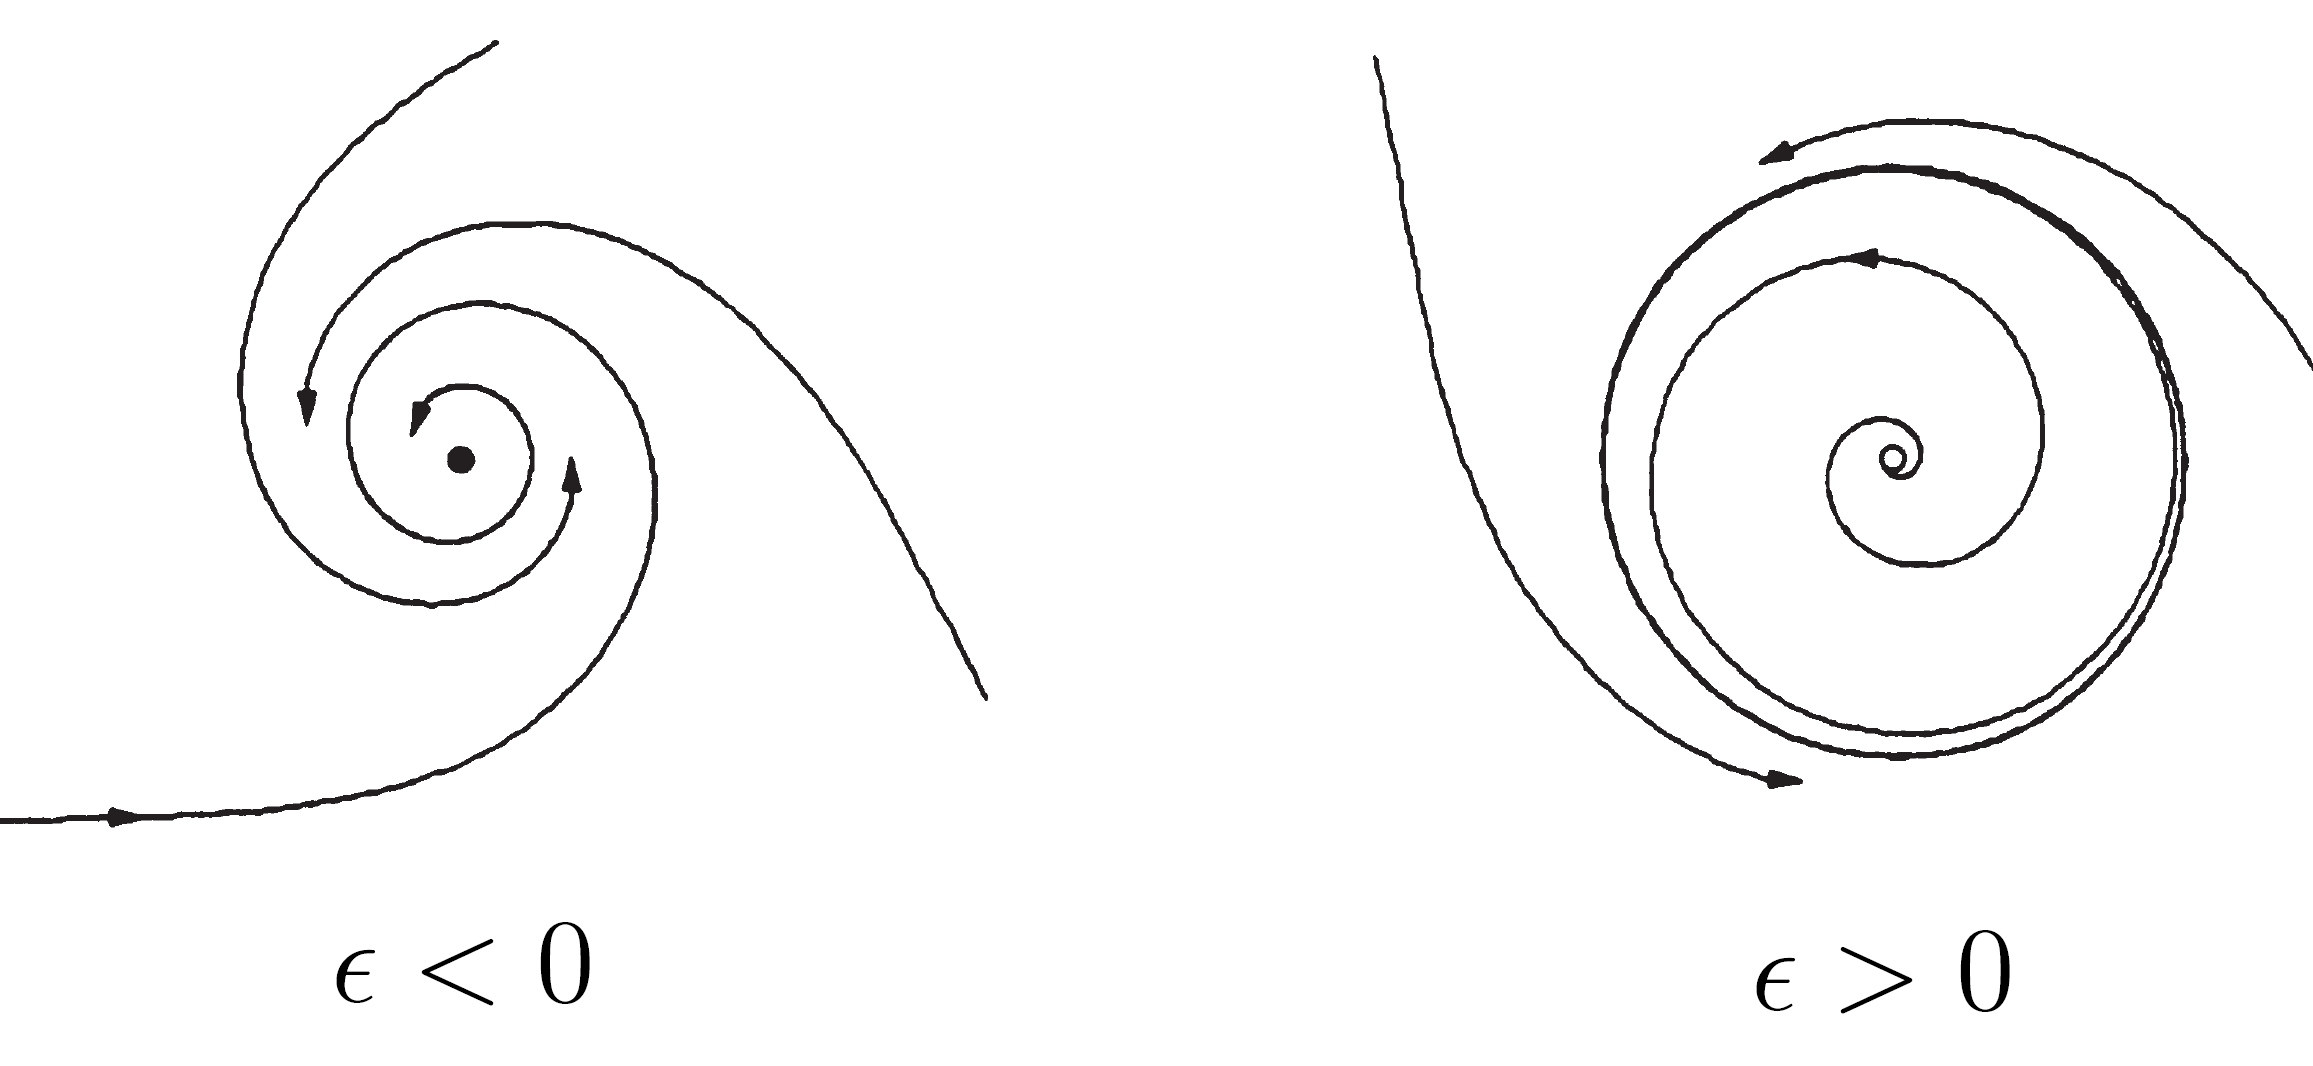
\includegraphics[width=\linewidth]{sphbf.png}
	\caption{Supercritical Hopf bifurcation}
	\label{fig:sphbf}
	\end{subfigure}
	\vline
	\begin{subfigure}{0.354\linewidth}
	\centering
	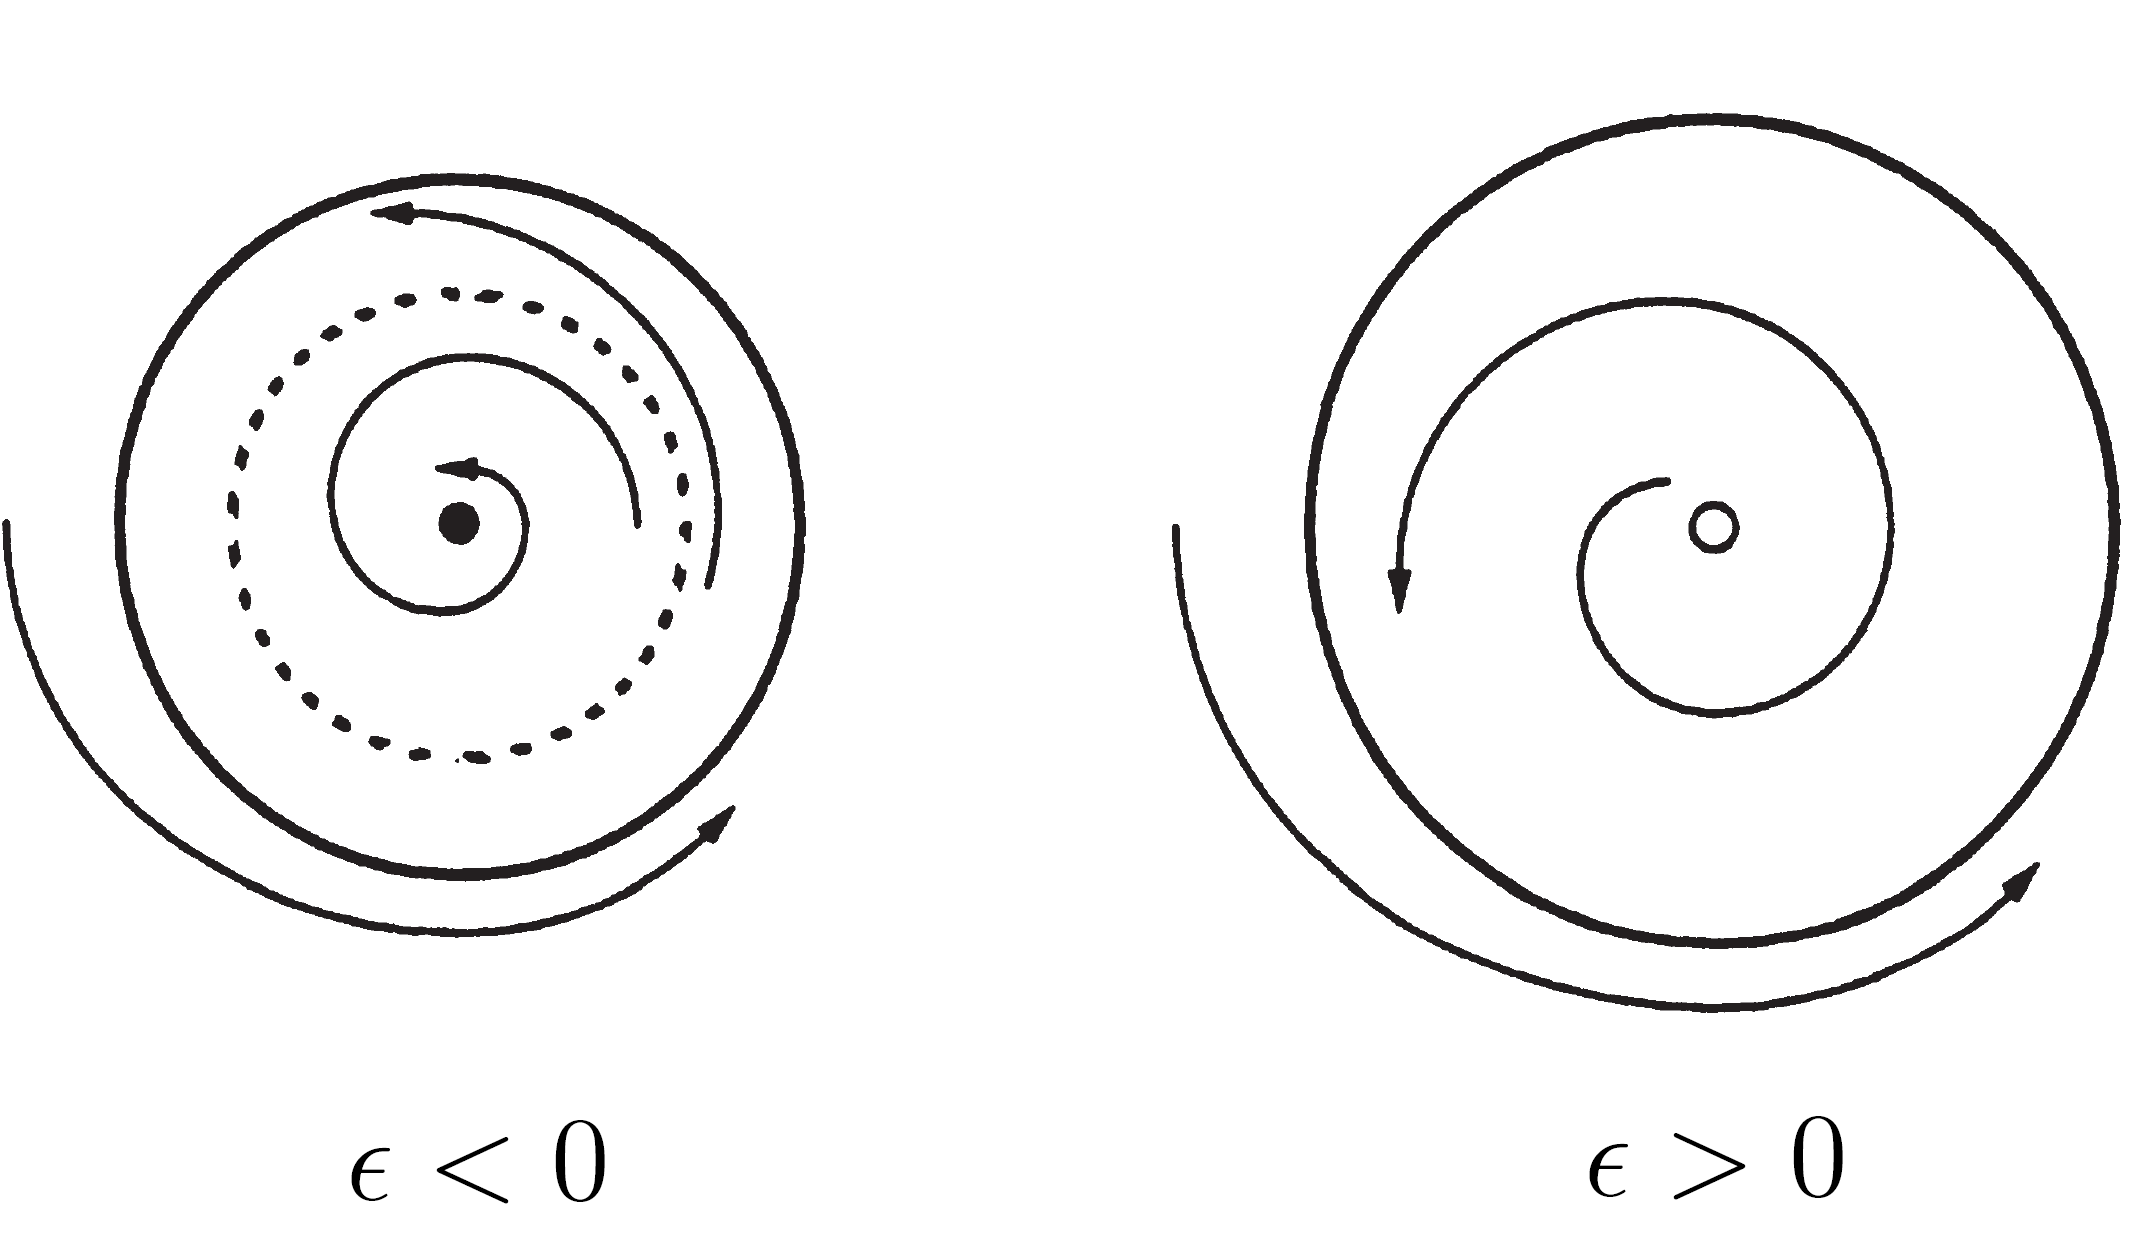
\includegraphics[width=\linewidth]{sbhbf.png}
	\caption{Subcritical Hopf bifurcation}
	\label{fig:sbhbf}
	\end{subfigure}
	\end{figure}
\end{comment}
A Supercritical Hopf bifurcation occurs when a stable spiral changes into an unstable spiral surrounded by a small, nearly elliptical limit cycle (Figure (\ref{fig:sphbf})).
\subsubsection{Subcritical Hopf Bifurcation}
Consider
\begin{equation}{\label{eq:sbhbf}}
	\begin{aligned}
		\dot{r}&=\epsilon r+2r^3-r^5\\
		\dot{\varphi}&=\omega
	\end{aligned}
\end{equation}
The fixed points are given by
\begin{equation}
	\tilde{r}_1=0\quad\tilde{r}_{2,3}^2=1\pm\sqrt{1+\epsilon}
\end{equation}
\begin{figure}[h!]
	\centering
	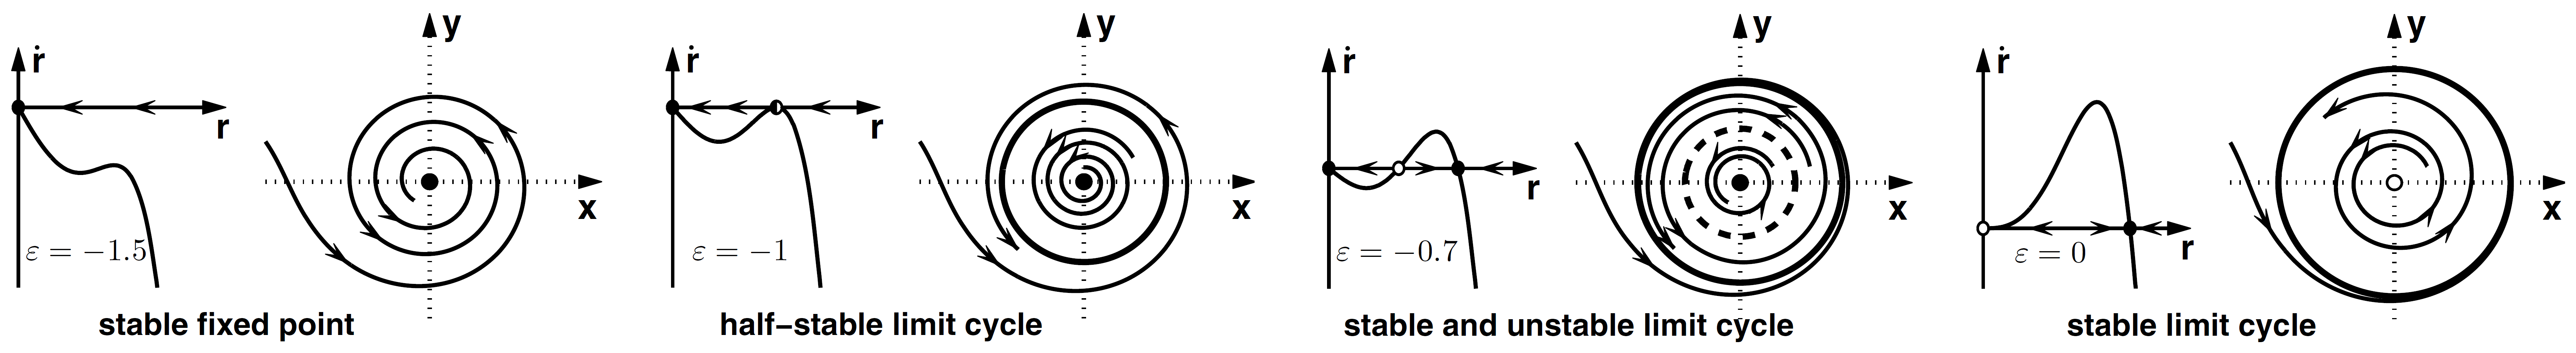
\includegraphics[width=\linewidth]{sbhbf2.png}
	\caption{Bifurcation sequence for the subcritical Hopf bifurcation.}
	\label{fig:sbhbf}
\end{figure}
For $\epsilon<-1$ (top left) $r_1=0$ is the only real solution of (\ref{eq:sbhbf}) and all trajectories spiral towards the origin, which is a stable fixed point.
At $\epsilon=-1$ (top right) a half-stable limit cycle exists where trajectories from the outside are attracted onto it and trajectories on the inside are repelled and evolve towards the origin.
For $-1<\epsilon<0$ the phase space plot in Figure (\ref{fig:sbhbf}) (bottom left) contains a stable fixed point at the origin and two limit cycles.
The inner limit cycle with a radius $r=\sqrt{1-\sqrt{1+\epsilon}}$ is unstable with trajectories moving away towards the still stable fixed point at the origin and a stable limit cycle with $r=\sqrt{1+\sqrt{1+\epsilon}}$.
At $\epsilon=0$ the unstable limit cycle and the stable fixed point at the origin collide, leaving a system with a single stable orbit with radius $r=\sqrt{2}$ and an unstable fixed point at the origin as shown in Figure (\ref{fig:sbhbf}) (bottom right).
\subsection{Global Bifurcations}
Global bifurcations occur when \emph{larger invariant sets}, such as \emph{periodic orbits}, collide with equilibria.
This causes changes in the topology of the trajectories in the phase space which cannot be confined to a small neighbourhood, as is the case with local bifurcations.
In fact, the changes in topology extend out to an arbitrarily large distance (hence \emph{global}).
\subsubsection{Infinite-Period Bifurcation}
Consider the system
\begin{equation}
	\begin{aligned}
		\dot{r}&=r(1-r^2)\\
		\dot{\theta}&=\mu-\sin\theta
	\end{aligned}
	\quad\text{where}\quad\mu\geq0
\end{equation}
In the radial direction, all trajectories (except $\tilde{r}=0$) approach the unit circle monotonically as $t\rightarrow\infty$.
In the angular direction, the motion is everywhere counterclockwise if $\mu>1$, whereas there are two invariant rays defined by $\sin\theta=\mu$ if $\mu<1$. As $\mu$ decreases, the limit cycle $r=1$ develops a bottleneck at $\theta=\pi/2$ that becomes increasingly severe as $\mu\rightarrow1^+$.
The oscillation period lengthens and finally becomes infinite at $\mu_c=1$, when a fixed point appears on the circle; hence the term \emph{infinite-period bifurcation}.
For $\mu<1$, the fixed point splits into a saddle and a node.
\begin{figure}[h!]
	\centering
	\begin{subfigure}{0.27\linewidth}
		\centering
		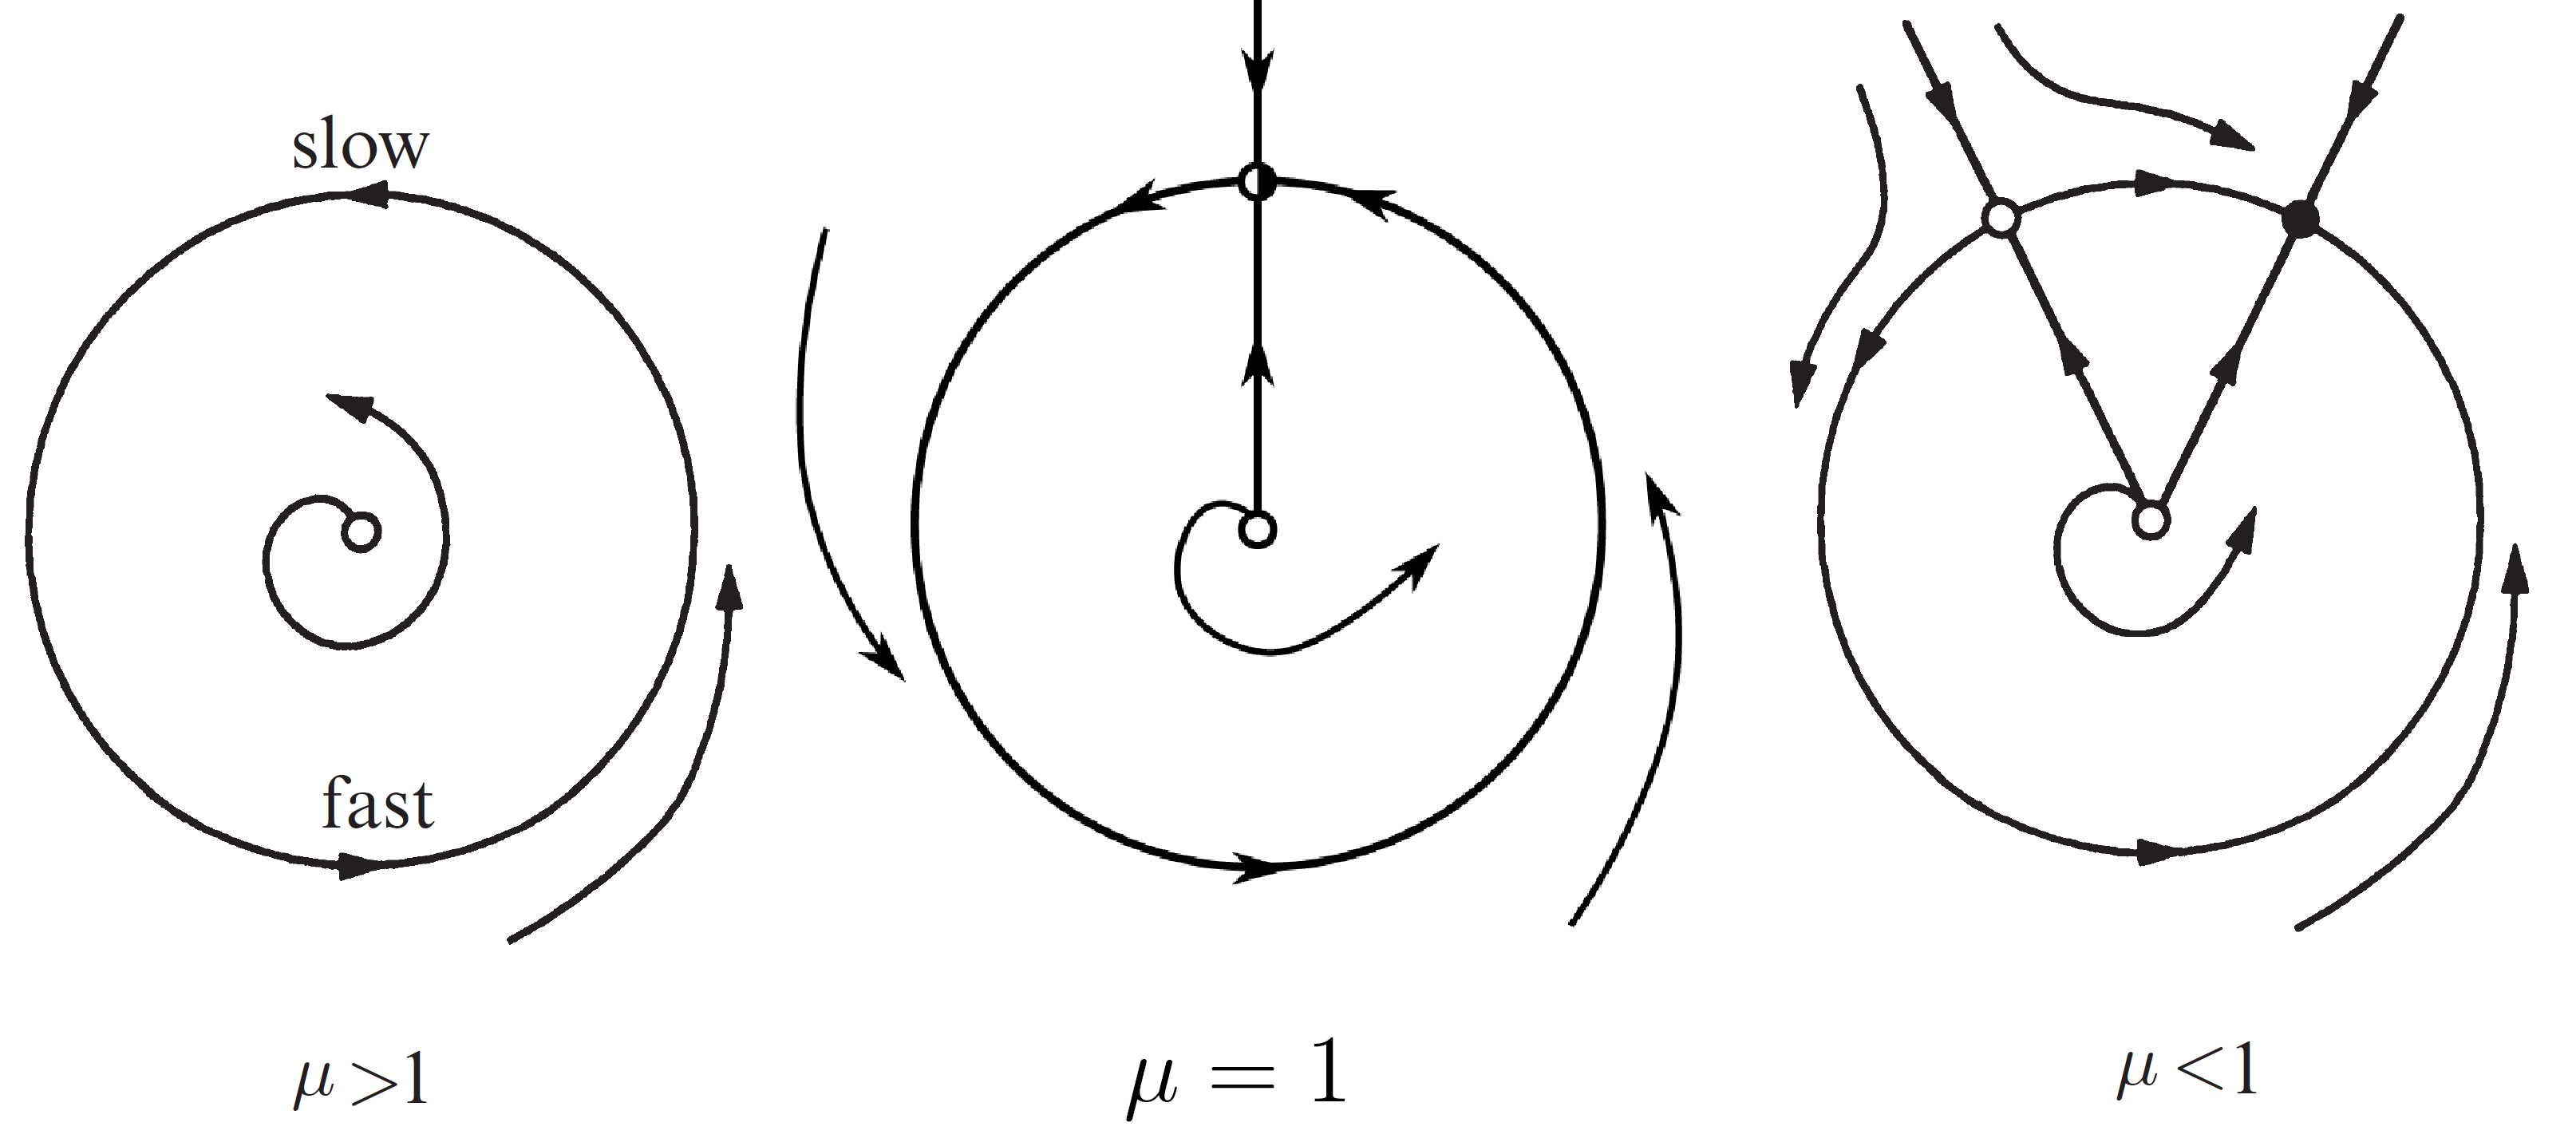
\includegraphics[width=\linewidth]{ipbf.png}
		\caption{Infinite-Period\\Bifurcation}
		\label{fig:ipbf}
	\end{subfigure}
	\vline
	\begin{subfigure}{0.7\linewidth}
		\centering
		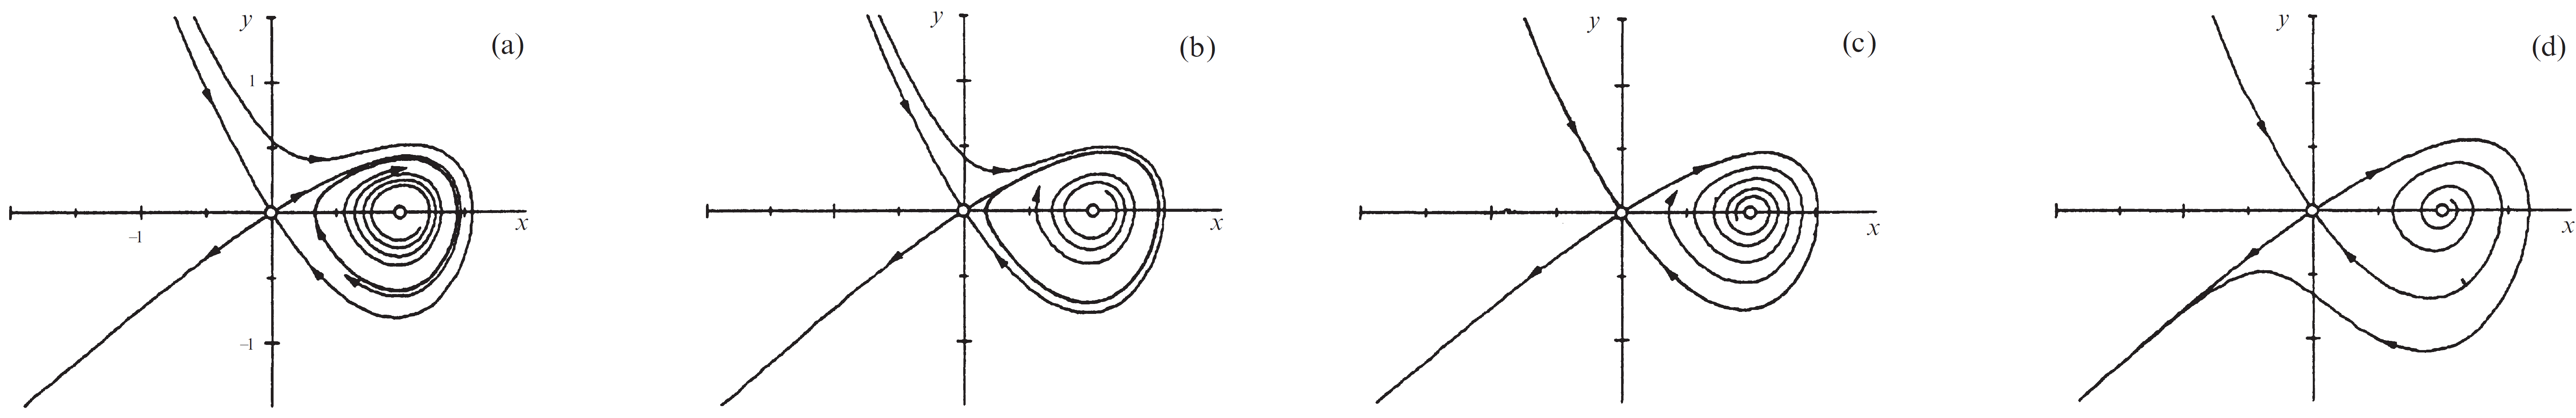
\includegraphics[width=\linewidth]{hcbf.png}
		\caption{Homoclinic Bifurcation}
		\label{fig:hcbf}
	\end{subfigure}
	\caption{}
\end{figure}
\subsubsection{Homoclinic Bifurcation}
Consider the system
\begin{equation}
	\begin{aligned}
		\dot{x}&=y\\
		\dot{y}&=\mu y+x-x^2+xy
	\end{aligned}
\end{equation}
Numerically, the bifurcation is found to occur at $\mu_c\approx-0.8645$. For $\mu<\mu_c$, say $\mu=-0.92$, a stable limit cycle passes close to a saddle point at the origin (Figure (\ref{fig:hcbf}a)).
As $\mu$ increases to $\mu_c$, the limit cycle swells (Figure (\ref{fig:hcbf}b)) and bangs into the saddle, creating a homoclinic orbit (Figure (\ref{fig:hcbf}c)).
Once $\mu>\mu_c$, the saddle connection breaks and the loop is destroyed (Figure (\ref{fig:hcbf}d)).
\subsubsection{Heteroclinic Bifurcation}
Here, a limit cycle collides with two or more saddle points.\\
This type of bifurcation will result in the change of stability of the heteroclinic cycle.
\paragraph{Resonance Bifurcations}
The stability of the cycle changes when an algebraic condition on the eigenvalues of the equilibria in the cycle is satisfied.
This is usually accompanied by the \emph{birth} or \emph{death} of a \emph{periodic orbit}.
\paragraph{Transverse Bifurcation}
It is caused when the real part of a transverse eigenvalue of one of the equilibria in the cycle passes through zero.
\subsubsection{Crisis}
A \textbf{crisis} is the sudden appearance or disappearance of a strange attractor as the parameters of a dynamical system are varied.
It occurs when a chaotic attractor comes into contact with an unstable periodic orbit or its stable manifold.
\paragraph{Exterior Crisis}
The attractor is suddenly \emph{destroyed} as the parameters are varied.
In the postbifurcation state the motion is transiently chaotic, moving chaotically along the former attractor before being attracted to a fixed point, periodic orbit, quasiperiodic orbit, another strange attractor, or diverging to infinity.
\paragraph{Interior Crisis}
The \emph{size} of the chaotic attractor suddenly \emph{increases}.
The attractor encounters an unstable fixed point or periodic solution that is inside the basin of attraction.
\paragraph{Attractor Merging Crisis}
Two or more chaotic attractors \emph{merge} to form a single attractor as the critical parameter value is passed.